% !TeX root = ../main.tex
% Add the above to each chapter to make compiling the PDF easier in some editors.

\chapter{Experiment setup and Methodology}\label{chapter:experiment_setup}
In this chapter we will discuss about our experiment setup and methodology for training our neural network models. Our goal is to preprocess the data from our simulation software in a format that we can feed it to the neural network models, then train the models. The data we got from our simulation is not suitable for direct feeding to the neural network because different models have different structure for the input of the data. We will also discuss the mythology behind the formatting of the data and our experiment setup and also the architectures of our Convolutional Neural Network (CNN).


\section{Data Preprocessing}

Our data preprocessing mainly contain 2 steps. First align the IMU data points (number of rows) according to the data points of our Ground Truth. Then fine tune the data in order to make it suitable for calculation of the CNN.

\subsection{Aligning the data rows}

As mention before in the section \ref{dataCollection} we took our IMU data and Ground Truth data in different files. For each IMU we have 2 files for accelerometer data from the accelerometer sensor and angular velocity data from the gyroscope. The Ground Truth data has one file for each simulation run.  The first thing is to check is the now of rows we got from each file. Our goal is to ensure that the count of data rows in the acceleration and angular velocity files was identical to the count of data rows in the GT file to ensure that they were fed smoothly into the model and keep the data sync with timestamps. Also, we wanted to ensure there are no “NaN” values in the data set to ensure that our model could learn optimally.

Our target was to get 100 thousand data rows. For that, we needed to run the simulation for more than an hour. We were expecting to get the same number of data rows from each file but unfortunately, that was not the case. We have a similar number of data rows form each IMU accelerometer and gyroscope, but the GT data rows were a bit less than the number of data rows from the IMU. For example, if we get ‘n’ number of data rows from each IMU file we were getting ‘n-x’ number of data rows from the GT.

Our assumption behind this problem is that when we stop the simulation by clicking the stop button The whole simulation doesn’t stop immediately. The plane stop moving but the Sensor still keeps generation some data on the other hand the GT stop generation data the moment we click stop because the GT script is a nested script, unlike the IMU script.
To overcome this problem, we used a simple solution.  We simply removed x data points from the data files of the accelerometer and the gyroscope to make all data files compatible with the same data point count. We measured the value of x is approximately 0.04\% of all data points which is ignorable.


\subsection{Data Tuning}

The next task is to tune the data in way that its suitable for feeding into the neural network model. Our simulation generated data is a numerical value consists variable number of digit after decimal point. We tried to feed the data into neural networks, but it prevented us from achieving optimal accuracy with many digits after the decimal point. The predicted values are not counted as a correctly forecast value because of small change in a given digit. We rounded up each data values to 4 digit after decimal point which gives us a small advantage in the accuracy of prediction and evaluation of the overall model.

% Please add the following required packages to your document preamble:
% \usepackage{graphicx}
% \usepackage[table,xcdraw]{xcolor}
% If you use beamer only pass "xcolor=table" option, i.e. \documentclass[xcolor=table]{beamer}
\begin{table}[h]
\centering
\resizebox{\textwidth}{!}{%
\begin{tabular}{|l|l|l|l|l|l|l|}
\hline
\rowcolor[HTML]{C0C0C0} 
\cellcolor[HTML]{9B9B9B}        & tx           & ty          & tz          & ox          & oy          & oz           \\ \hline
\cellcolor[HTML]{C0C0C0}Row n   & -0.187795669 & 1.460141063 & 0.024999999 & 0.006407991 & 1.227231145 & -0.063147597 \\ \hline
\cellcolor[HTML]{C0C0C0}Row n+1 & -0.189894766 & 1.461498737 & 0.024999999 & 0.023488231 & 1.222845793 & -0.069066621 \\ \hline
\end{tabular}%
}
\caption{Sample ground truth data before rounding up}
\label{tab: gtBR}
\end{table}

% Please add the following required packages to your document preamble:
% \usepackage{graphicx}
% \usepackage[table,xcdraw]{xcolor}
% If you use beamer only pass "xcolor=table" option, i.e. \documentclass[xcolor=table]{beamer}
\begin{table}[]
\centering
\resizebox{\textwidth}{!}{%
\begin{tabular}{|c|c|c|c|c|c|c|}
\hline
\rowcolor[HTML]{CBCEFB} 
                                         & \textbf{tx} & \textbf{ty} & \textbf{tz} & \textbf{ox} & \textbf{oy} & \textbf{oz} \\ \hline
\cellcolor[HTML]{CBCEFB}\textbf{Row n}   & -0.1877     & 1.4602      & 0.0250      & 0.0065      & 1.2273      & -0.0631     \\ \hline
\cellcolor[HTML]{CBCEFB}\textbf{Row n+1} & -0.1898     & 1.4615      & 0.0250      & 0.0235      & 1.2229      & -0.0690     \\ \hline
\end{tabular}%
}
\caption{Sample ground truth data after rounding up}
\label{tab: gtAR}
\end{table}


Table \ref{tab: gtBR} and Table \ref{tab: gtAR} show the effect of change when the values are rounded. The new data looks better and we were able to test our models more effectively.





\section{Methodology for processing data for the input}

As our ground truth data values provide us with the pure pose (position and orientation) of the object. To train our model we wanted to predict the difference of pose for a particular timestamp using the previous timestamp data from the sensors (IMUs). For example, for time t\textsubscript{0} we have the object pose pt\textsubscript{0}. In time t\textsubscript{1}­­­ we will have the object pose pt\textsubscript{1} so our pose change from time t\textsubscript{0} to t\textsubscript{1} ( $\Delta$ t ) will be $\Delta$ p.
We want to predict this delta p using the IMU data at time t\textsubscript{0} and t\textsubscript{1}.  It became obvious when we see the equation for velocity, acceleration, and angular velocity.

\begin{equation}
vt = vt_{0}  + a* \Delta t  \label{eq:6.1}
\end{equation}

equation \ref{eq:6.1} is the standard equation for the velocity of an object in time t.  where vt\textsubscript{0} is the velocity in time t\textsubscript{0} and a is the acceleration and delta t = t\textsubscript{1} -t\textsubscript{0} .

\begin{equation}
  a = \frac{v\textsubscript{t} - vt\textsubscript{0}} {\Delta t}  \label{eq:6.2}
\end{equation}

from equation  \ref{eq:6.2} we can see that acceleration depends on the time delta and the velocity delta.


\begin{equation}
p\textsubscript{t} = p\textsubscript{t0}  + v\textsubscript{t}  \label{eq:6.3}
\end{equation}

Equation  \ref{eq:6.3} is the standard equation for the calculation position at time t. 


\begin{equation}
s = v * t  \label{eq:6.4}
\end{equation}

\begin{equation}
\Omega = \frac {v} {r}  \label{eq:6.5}
\end{equation}

Equation  \ref{eq:6.4} , which also depends on velocity, is the standard equation for distance. Equation  \ref{eq:6.5}  is the normal angular-speed expression, which depends also on the distance. R in this equation, the radius is indicated if the circle created at that time. It gave us the concept of using time differences (always) between two data points rather than the actual time. Using the following basic equation, we replace the raw time (in milliseconds) of our data using time delta.

\begin{equation}
  \Delta t = t_{i+1} - t\textsubscript{1}  \label{eq:6.6}
\end{equation}

We have decided to use the position delta as our labels because we calculate the time frame differences. This applies to the position and orientation of the object, the plane in our case. This helps us to assess how much displacement in a given time interval has been made in the position and orientation of the plane. The fact is that, instead of the actual position and orientation values in time, it makes more sense to calculate the difference. Since orientation and position may have similar values at different timestamps.We used Equation  \ref{eq:6.6} to get the time difference.

\begin{equation}
  \Delta p= p\textsubscript{i+1} - t\textsubscript{1}  \label{eq:6.7}
\end{equation}

\begin{equation}
  \Delta o= o\textsubscript{i+1} - o\textsubscript{1}  \label{eq:6.8}
\end{equation}

Equation \ref{eq:6.7} and  \ref{eq:6.8} represent the method of measuring position and orientation displacements. By following this method, we feed displacements as labels to the neural networks. The network will predict the displacements after the training is complete. The Euclidian distance can also be calculated.


\section{Convolutional Neural Network Architecture}


We use various combinations of architecture to evaluate our solution. We created the combinations based on the different hidden layers, number of neurons, number of channels in the input layer. We obviously played with the different hyperparameter for each architecture to make its performance better but we did not see as a major architectural difference. We will describe the hyperparameter at the index <()>.

\begin{figure}[h]
  \centering
    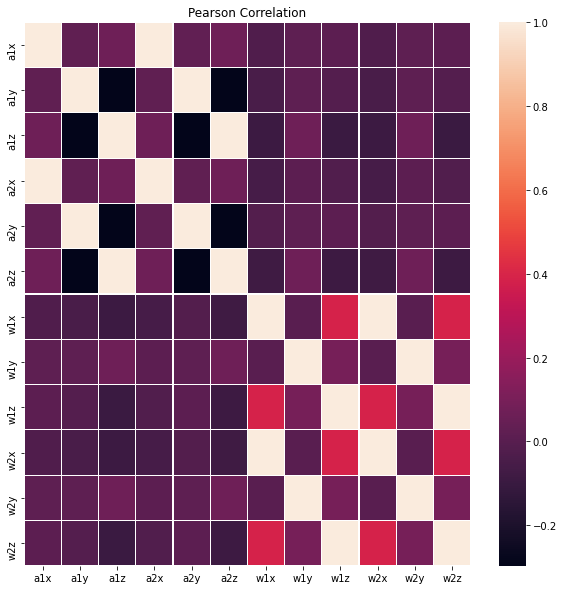
\includegraphics[width=0.5\linewidth]{figures/dataCorelation.png}
    \caption{Pearson correlation of IMU-2 dataset.}
\label{fig:dataCorelation}
\end{figure}

Before we discuss our CNN architecture we wanted to check if our dataset is suitable for regression analysis as we do not have the problem of multiple variables depending on each other or in other words, multi-colinearity.  For that, we did Pearson correlation to visualize the correlation among the variables in our dataset. From the figure \ref{fig:dataCorelation} we can see that our data does not have that problem.

Our basic CNN architecture starts with a (w * h) input layer then 'n' hidden CNN layer and the output is always a dense layer with 6 neurons as we need the output of 6 data points.
It is important to note that, instead of the 2D convolution layer we used the 1D convolution layer because the 2D convolution works very well for image and video data where 1D convolution is best suitable for time series data. The main difference between 1D and 2D convolution is that in 1D convolution the kernel slides along one dimension wherein 2D convolution the kernel slides along 2 dimensions (width and height)

The figure \ref(fig:diff1D2D) shows the difference between 1d and 2d convolution

\begin{figure}[h!]
  \centering
  \begin{subfigure}[b]{0.4\linewidth}
    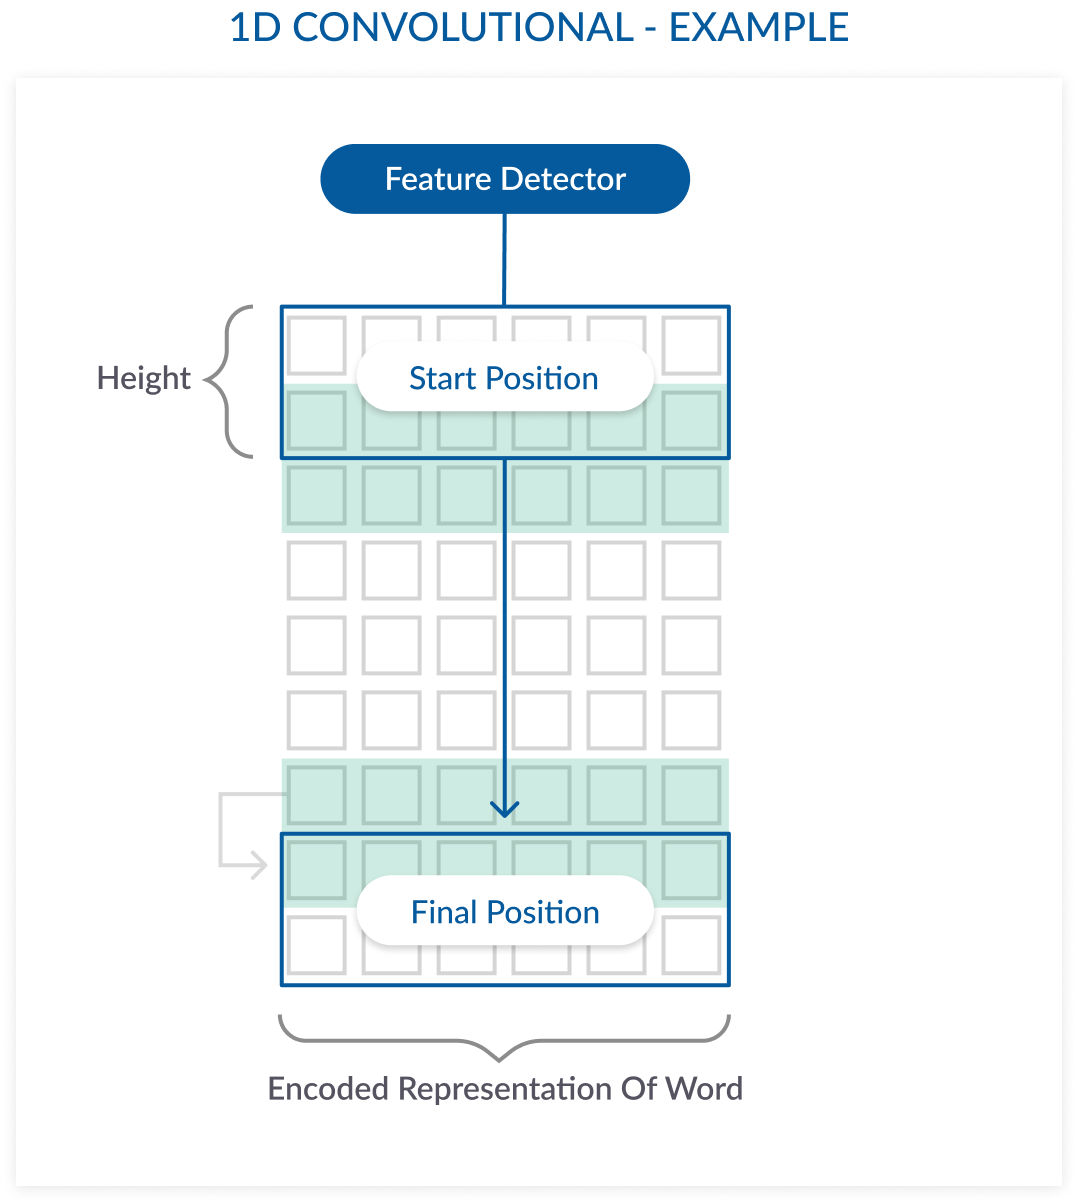
\includegraphics[width=\linewidth]{figures/1Dconv.png}
    \caption{1D convolution architecture}
  \end{subfigure}
\quad
\begin{subfigure}[b]{0.4\linewidth}
    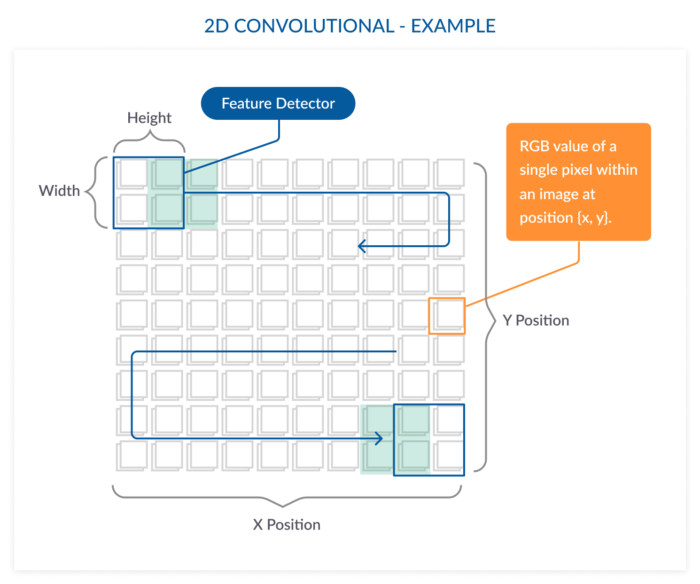
\includegraphics[width=\linewidth]{figures/2Dconv.png}
    \caption{2D convolution architecture}
  \end{subfigure}
 \caption{Difference between 1D and 2D convolution.}
  \label{fig:diff1D2D}
\end{figure}

We can divide our CNN architecture into two major categories Expanding model and Shirking model. As the name suggests the expanding model increases the number of neurons for each layer and the shirking model decreases the number of neurons for each layer. For each shrinking and expanding model we also experiment with different numbers of hidden layers.
For example, the shrinking model we had 2 convolution layers and 3 convolution layers the same with the expanding model. The figure shows the visual representation of the shrinking and expanding models of 2 convolutional layer.


\begin{figure}[h!]
  \centering
  \begin{subfigure}[b]{\linewidth}
    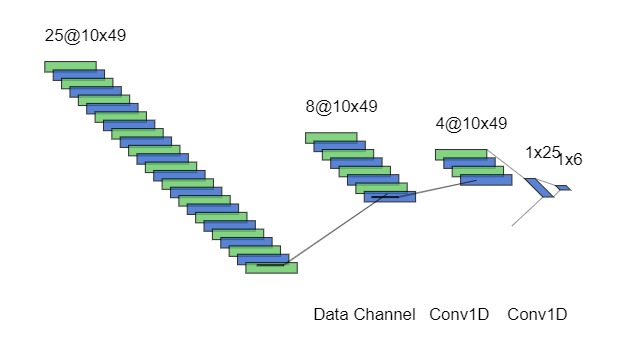
\includegraphics[width=\linewidth]{figures/shrinkingModel.png}
    \caption{Shrinking model architecture  }
  \end{subfigure}
\quad
\begin{subfigure}[b]{\linewidth}
    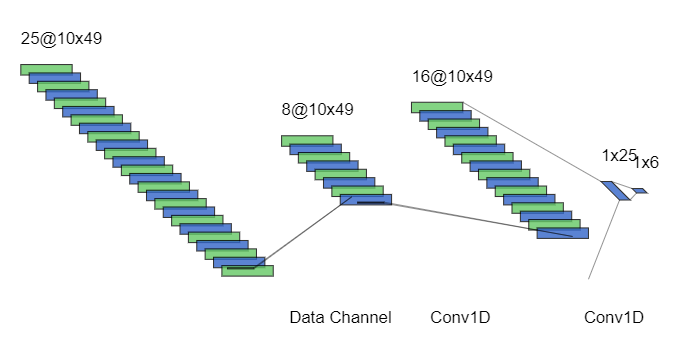
\includegraphics[width=\linewidth]{figures/expandModel.png}
    \caption{Expanding  model architecture}
  \end{subfigure}
 \caption{Visual representation of shrinking expanding model architecture.}
  \label{fig:vsExSr}
\end{figure}

We did not use dropout in our architecture mainly because dropout usually used to prevent overfitting and it turns off some neuron to do that. Because of that, some data might not get calculated in the CNN. In our situation, we are not finding features from our data so that we can not prioritize some sections and drop some sections of data in the calculation. Instead of dropout, we used batch normalization to overcome the problem of overfitting


\section{CNN Parameters}
will be discueed

\section{Loss Function}
A typical neural network is developed by stochastic gradient optimization algorithms and weights modified by algorithm back propagation. The word 'gradient' is a gradient of mistake. The loss function or target function is used to evaluate the solutions for the candidate during optimisation. The goal is to minimize the error and the function is called a loss or cost function.Since our problem is a regression problem, there are two viable loss functions to optimize our algorithms. Mean Absolute Error (MAE) and Mean Squared Error (MSE). 


Yi is the real label value of these equations, and (y i) da is the value expected. Such two failure features have their own benefits and disadvantages. For MAE, if there are more outliers it works better because there are no square operations. Average all distances. On the other side, since there is a square procedure MSE penalizes long distances. For broad values, MSE has a higher gradient. MAE contribute to cost optimisation and therefore to the network's constant learning speed. For MSE, that's quite the opposite. Our dataset includes not so many outliers, so MSE performed on our unique dataset more effectively. This doesn't mean MAE can't be done at all. This doesn't mean MAE can't be done at all. For MSE we performed in terms of training time and predictive efficiency a little better.

\section{Optimizer}
One of the arguments needed to compile a model in Keras is an optimizer. An significant parameter since optimizers determine how the cost function of neural networks is the. The goal is to find the minimum. For neural networks there are many optimizers available, such as –Stochastic Gradient Descent (SGD), Root Mean Square Propagation (RMSProp), Adaptive Moment Estimation (Adam), Nesterov-accelerated Adaptive Moment Estimation (Nadam) ) and others. The goal is to find the global minimum at which the learning cost is the lowest.
Although the gradient decent attempts to optimize the cost or loss function without updating the weight deviation, it could hover over the optimal values instead. Via its capacity to change the weight at every data point, the solution is therefore to use SGD. SGD is problem-sensitive too, however, since the batch size is too big to predict right. SGD's Mini-batch SGD and SGD had implemented a momentum in order to overcome this problem. There is even an acceleration parameter which supports SGD in its optimization.Yet weight-update gets very fast when dynamic and speed-up are mixed, confounding and anticipating the network. A comparatively better solution is Adagrad, which is able to update weights for every parameter in a very good direction. The learning rate parameter will then decrease to a point in which the parameters are no longer changed and the learning process will end. 

Adam for deep learning is one of the most commonly used and effective optimizers. This is close to the method by which the optimizer adds momentum. The learning process seems slow at the beginning, but it gets faster after some time. For various parameters to change Adam may also take a different time step. It leads to faster convergence with the help of momentum. Since Adam is a common optimizer, we decided to adjust the learning rate for Adam over SGD with the default adam parameters. We agreed in several iterations to use a chart of leaning rates for a single standard.
We chose to use a list of leaning rate for a single model in multiple iterations.

lr = [0.01, 0.001, 0.0001]

Initially all the other parameters of adam such as – beta1, beta2, epsilon, decay were remained with the default values. 

\section{Data structure for CNN}

We decided to use a number of different data channel for the input layer, Our main motivation was to determine how many rows of sensor data is needed to predict accurately the pose. Our initial approach was to use every row of input data (IMU) to predict every row of pose data (GT).
(table here)
But CNN doesn’t work that way. CNN models try to convolute the data and try to find the best feater in the data set for that purpose 1 by 1 approach don’t work. Then we decided to divide the data into channels. For example, we used n number of data rows to predict 1 pose. Here n could be 2, 5, 10, and 20, if we used 5 rows of IMU data as an input channel then we tried to predict the 6th row of pose (data).  As in for every 5n data rows for the input we try to predict (5n+1)th row of pose data
The image below shows the data channel. We used this method for 10n, 15n and 20n to determine the optimal data channel
It's very important to note that we used this architecture to train our model for 2, 4, 8 and16  IMU.